\documentclass[aspectratio=43, 10pt]{beamer}
\usetheme{metropolis}
\setbeamertemplate{page number in head/foot}[totalframenumber]

\usepackage[spanish]{babel}
\usepackage{amsmath}
\usepackage[backend=biber,style=apa,sortcites,natbib=true]{biblatex}
\usepackage{multirow}
\usepackage{ragged2e}
\usepackage{tabularx}

\addbibresource{../doc-udelar/bibliografia/tesis.bib}
\addbibresource{../doc-udelar/bibliografia/ambicycle.bib}

\usefonttheme[onlymath]{serif}

\newcommand{\argmin}{\mathop{\mathrm{argmin}}}
\newcommand{\modelspace}{\hspace{1.5em}}

\title{Diseño de redes de ciclovías enfocado a la atracción de demanda}
\subtitle{Maestría en Investigación de Operaciones}

\author{
    \textbf{Joaquín Correa} \\\\
    \and
    Director Académico: Franco Robledo \\
    \and
    Directores de Tesis: Antonio Mauttone y Franco Robledo \\
}

\institute{Facultad de Ingeniería, Universidad de la República}
\date{Agosto 2022}

\begin{document}
\frame{
    \titlepage
}

\begin{frame}
    \frametitle{Resumen y motivación}

    \begin{itemize}
    \item{Trabajo en el marco del transporte público}
    \item{Atracción de demanda entre modos de transporte (hacia la bicicleta)}
    \item{Beneficios de trasladarse en bicicleta para personas y para las ciudades}
    \item{Problema modelado utilizando programación matemática}
    \item{Dos entidades: planificador y usuarios}
    \item{Pruebas con datos de la ciudad de Montevideo}
    \end{itemize}
\end{frame}

\begin{frame}
    \frametitle{Contenido}
    \tableofcontents
\end{frame}

\section{Bibliografía}

\begin{frame}
    \frametitle{Bibliografía - Conceptos}

    \begin{itemize}
    \item{Red}
    \item{Ciclovía}
    \item{Demanda}
    \item{Camino más corto}
    \item{Costo de usuario}
    \item{Costo de construcción}
    \end{itemize}
\end{frame}

% \subsection{Diseño de ciclovías}

\begin{frame}
    \frametitle{Bibliografía - Diseño de ciclovías}

    Problemas abordados con programación matemática con variantes.

\begin{itemize} \item{
        Algunos objetivos:
        \begin{description}
        \item[Costo de construcción] \parencite{Duthie2014}
        \item[Costo (Utilidad) de usuario] \parencite{Mauttone2017, Liu2019, baya2021}
        \item[Penalizar cambios de tecnologías de ciclovías] \parencite{baya2021}
        \end{description}
    }
    \item{
        Algunas restricciones:
        \begin{description}
        \item[Desvío máximo del camino más corto] \parencite{Duthie2014, lim2021}
        \item[Presupuesto]
        \end{description}
    }
    \item{
            Hipótesis
            \begin{description}
            \item[Existen diferentes tecnologías de ciclovías]\parencite{baya2021, Zhu2019}
            \item[Camino seguro] \parencite{Duthie2014, lim2021}
            \end{description}
    }
    \end{itemize}
\end{frame}

% \subsection{Transferencia de demanda}

\begin{frame}
    \frametitle{Bibliografía - Transferencia de demanda}

    % Dos enfoques:

    \begin{description}
        \item[Modelos probabilísticos] {
            valor esperado de uso de la bicicleta basándose en probabilidad de su utilización
            \parencite{ortuz2011, Liu2019, Pacheco2021}.

            \begin{equation*}
                P(bicicleta) = {e^{U_{bicicleta}} \over \sum_{t \in T} e^{U_t}}
            \end{equation*}
        }
        \item[Modelo determinista] {
            valor de viajes en bicicleta en función de las variables del modelo (costo de viaje)
            \parencite{marin2007, laporte2007}

            \begin{equation*}
                f(C) = \left\{ \begin{array}{lcr}
                D & \text{si}   & C \leq C_{min} \\
                  0 & \text{si no} &
            \end{array}
            \right.
            \end{equation*}
        }
    \end{description}
\end{frame}

% \subsection{Comportamiento de los usuarios}

\begin{frame}
    \frametitle{Bibliografía - Comportamiento de los usuarios}

    Usuarios ciclistas:

    \begin{itemize}
        \item{Prefiere rutas más tranquilas y seguras que rutas más cortas. \parencite{winters2010}}
        \item{No afectados por congestión. \parencite{Lin2013, Duthie2014} y otros}
        \item{Distancia de viaje promedio: 2,6 km y 3.0 km para bicicletas comúnes y eléctricas. \parencite{anette2018}}
    \end{itemize}

    Potenciales ciclistas \parencite{shwe2014}:

    \begin{itemize}
        \item{La sola presencia de ciclovías puede no incentivar el cambio}
        \item{Los viajes menores a 5 km son considerados realizables en bicicleta}
    \end{itemize}
\end{frame}

% \subsection{Utilización de la bicicleta}

\begin{frame}
    \frametitle{Bibliografía - Decisión de utilizar la bicicleta}

    Depende de varios factores \parencite{ortuz2011}:

    \begin{description}
        \item[Características del viajante] edad, nivel socioeconómico, situación familiar, trabajo.
        \item[Características del viaje] propósito, momento del día.
        \item[Características de las instalaciones] disponibilidad y costo del transporte público, disponibilidad de ciclovías, seguridad y protección al usar la bicicleta.
    \end{description}
\end{frame}

\begin{frame}
    \frametitle{Bibliografía - Diseño de redes}

    Problemas típicos de optimización en redes, tomados del libro \textcite{crainic2021}:

    \begin{description}
        \item[Fixed-Charge] ruteo de una o varias commodities sobre instalaciones con un costo fijo
        \item[Multi-Facility] ruteo de múltiples commodities sobre varios tipos de instalaciones
        \item[Bilevel] problemas compuestos por dos entidades jerárquicas no necesariamente alineadas
        \item[Piecewise linear costs] modelado de costos graduales en función de variables del modelo
    \end{description}
\end{frame}

\section{Definición del problema}

\begin{frame}
    \frametitle{Definición del problema}

    Buscamos un modelo que:

    \begin{itemize}
        \item{Maximice la demanda transferida a la bicicleta desde un modo de transporte}
        \item{Tome buenas decisiones sobre la red de ciclovías resultante}
    \end{itemize}

    Tomando como hipótesis que:

    \begin{itemize}
        \item{Usuarios buscan minimizar el costo de trasladarse entre origen y destino}
        \item{Tiempo de viaje en bicicleta es independiente del flujo}
        \item{Bicicletas pueden circular por las calles}
        \item{La construcción de ciclovías en un arco disminuye el costo de usuario de recorrerlo}
        \item{La disminución en el costo de usuario de trasladarse afecta la demanda que utiliza la bicicleta}
    \end{itemize}
\end{frame}

\begin{frame}
    \frametitle{Definición del problema - Modelo}

    Sean los siguientes conjuntos, parámetros y variables:

    \begin{description}
        \item[$OD$] conjunto de pares OD (commodities).
        \item[$I$] conjunto de tecnologías de ciclovías (facilities).
        \item[$G(N,A)$] grafo dirigido compuesto por nodos $N$ y arcos $A$.
        \item[$C_{ai}$] costo de usuario de recorrer un arco utilizando una tecnologías.
        \item[$H_{ai}$] costo de construir la tecnología sobre un arco.
        \item[$B$] presupuesto para construcción de ciclovías.
        \item[$y_{ai}$] variable binaria que decide si una tecnología está activa en un arco.
        \item[$x_{ak}$] variable continua que decide si el flujo de un par OD utiliza un arco.
    \end{description}
\end{frame}

\begin{frame}
    \frametitle{Definición del problema - Modelo (cont.)}

    \begin{align}
      \max_{w,x,y}   & \sum_{k \in OD} f_k(w_k)                                                         & \label{eq:objective1lvl} \\
      \text{s.t.}\;  & \sum_{a \in A} \sum_{k \in OD} \sum_{i \in I} C_{ai}y_{ai}x_{ak} = w_k           & \forall k \in OD \label{eq:shortestpath} \\
                     & \sum_{a \in A} \sum_{i \in I} H_{ai}y_{ai} \leq B                                & \label{eq:respectbudget} \\
                     & \sum_{i \in I} y_{ai} = 1                                                        & \forall a \in A \label{eq:alwaysoney} \\
                     & y_{ai} \in \{0,1\}                                                               & \forall a \in A, i \in I \nonumber \\
                     & x \in \argmin_{x'} \sum_{a \in A} \sum_{k \in OD} \sum_{i \in I} C_{ai}y_{ai}x'_{ak}  & \label{eq:subproblem} \\
                     & \qquad \text{s.t.} \sum_{a \in A_n^+} x'_{ak} - \sum_{a \in A_n^-} x'_{ak} = \theta_{nk}   & \forall n \in N, k \in OD \label{eq:flowbalance} \\
                     & \qquad \modelspace x'_{ak} \geq 0                                                          & \forall a \in A, k \in OD \nonumber
    \end{align}
\end{frame}

\section{Resolución}
% \subsection{Problema binivel}

\begin{frame}
    \frametitle{Resolución - Problema binivel}

    Metodología tomada de \textcite{bardbook}

    \begin{itemize}
        \item{BLPP continuo: NP-Hard. Nuestro modelo además tiene variables enteras}
        \item{Método más común: transformación a un MILP mediante condiciones de KKT del segundo nivel}
        \item{Existen algoritmos específicos basados en B\&B, Simplex, condiciones de KKT y heurísticas que pueden ser complejos sin ventajas claras sobre el anterior}
    \end{itemize}
\end{frame}

\begin{frame}
    \frametitle{Resolución - Reformulación a un problema MILP}

    Transformacion a MILP por método de KKT agrega más variables enteras, además de las $y_{ai}$ \parencite{kara2004}:
    \begin{itemize}
    \item{Para linealizar condiciones de KKT}
    \item{Flujos pasan a ser enteros porque se pierde la unimodularidad del problema de segundo nivel}
    \end{itemize}

    \vspace{10pt}

    Transformación propuesta: las $f_k$ son estrictamente decrecientes entonces maximizar demanda transferida implica minimizar el costo del camino de menor costo.
    \vspace{10pt}

    \begin{block}{Problema MILP}
        Problema de primer nivel + restricciones del problema de segundo nivel.
    \end{block}
\end{frame}

\begin{frame}
    \frametitle{Resolución - Reescritura de variables no lineales}
    Cálculo del costo de un camino según el tipo de ciclovía activa en cada arco (la restricción de balance de flujo se mantiene igual):

    \begin{columns}[c]
        \column{.5\textwidth}
            \begin{eqnarray*}
              \sum_{a \in A, i \in I} C_{ai} x_a y_{ai} \\
              x_a \geq 0 & \forall a \in A \\
              y_{ai} \in \{0,1\} & \forall a \in A, i \in I \\
            \end{eqnarray*}
            el producto $x_a y_{ai}$ modela el flujo por el arco $a$ usando la
            ciclovía $i$.
        \column{.5\textwidth}
            \begin{eqnarray*}
              \sum_{a \in A, i \in I} C_{ai} h_{ai} & \\
              h_{ai} \leq y_{ai} & \forall a \in A, i \in I \\
              h_{ai} \geq 0 & \forall a \in A, i \in I \\
              y_{ai} \in \{0,1\} & \forall a \in A, i \in I \\
            \end{eqnarray*}
            luego, $\sum_{i \in I} h_{ai} = x_{a}$
    \end{columns}
\end{frame}


\begin{frame}
    \frametitle{Resolución - Definición de funciones de transferencia}

    \begin{columns}[c]
        \column{.5\textwidth}
            \begin{itemize}
                \item{Modelado de funciones decrecientes}
                \item{Representadas como problema lineal}
                \item{Representación no es estrictamente decreciente}
            \end{itemize}
            \begin{align*}
              f(W) =\; & \max \sum_{j \in J} P_j z_j   & \\
                       & \;s.t. \sum_{j \in J} z_j = 1   & \\
                       & \qquad Q_j \geq W z_j         & \forall j \in J \\
                       & \qquad z_j \in \{0,1\}        & \forall j \in J
            \end{align*}
        \column{.5\textwidth}
            Ejemplo

            \vspace{.5cm}
            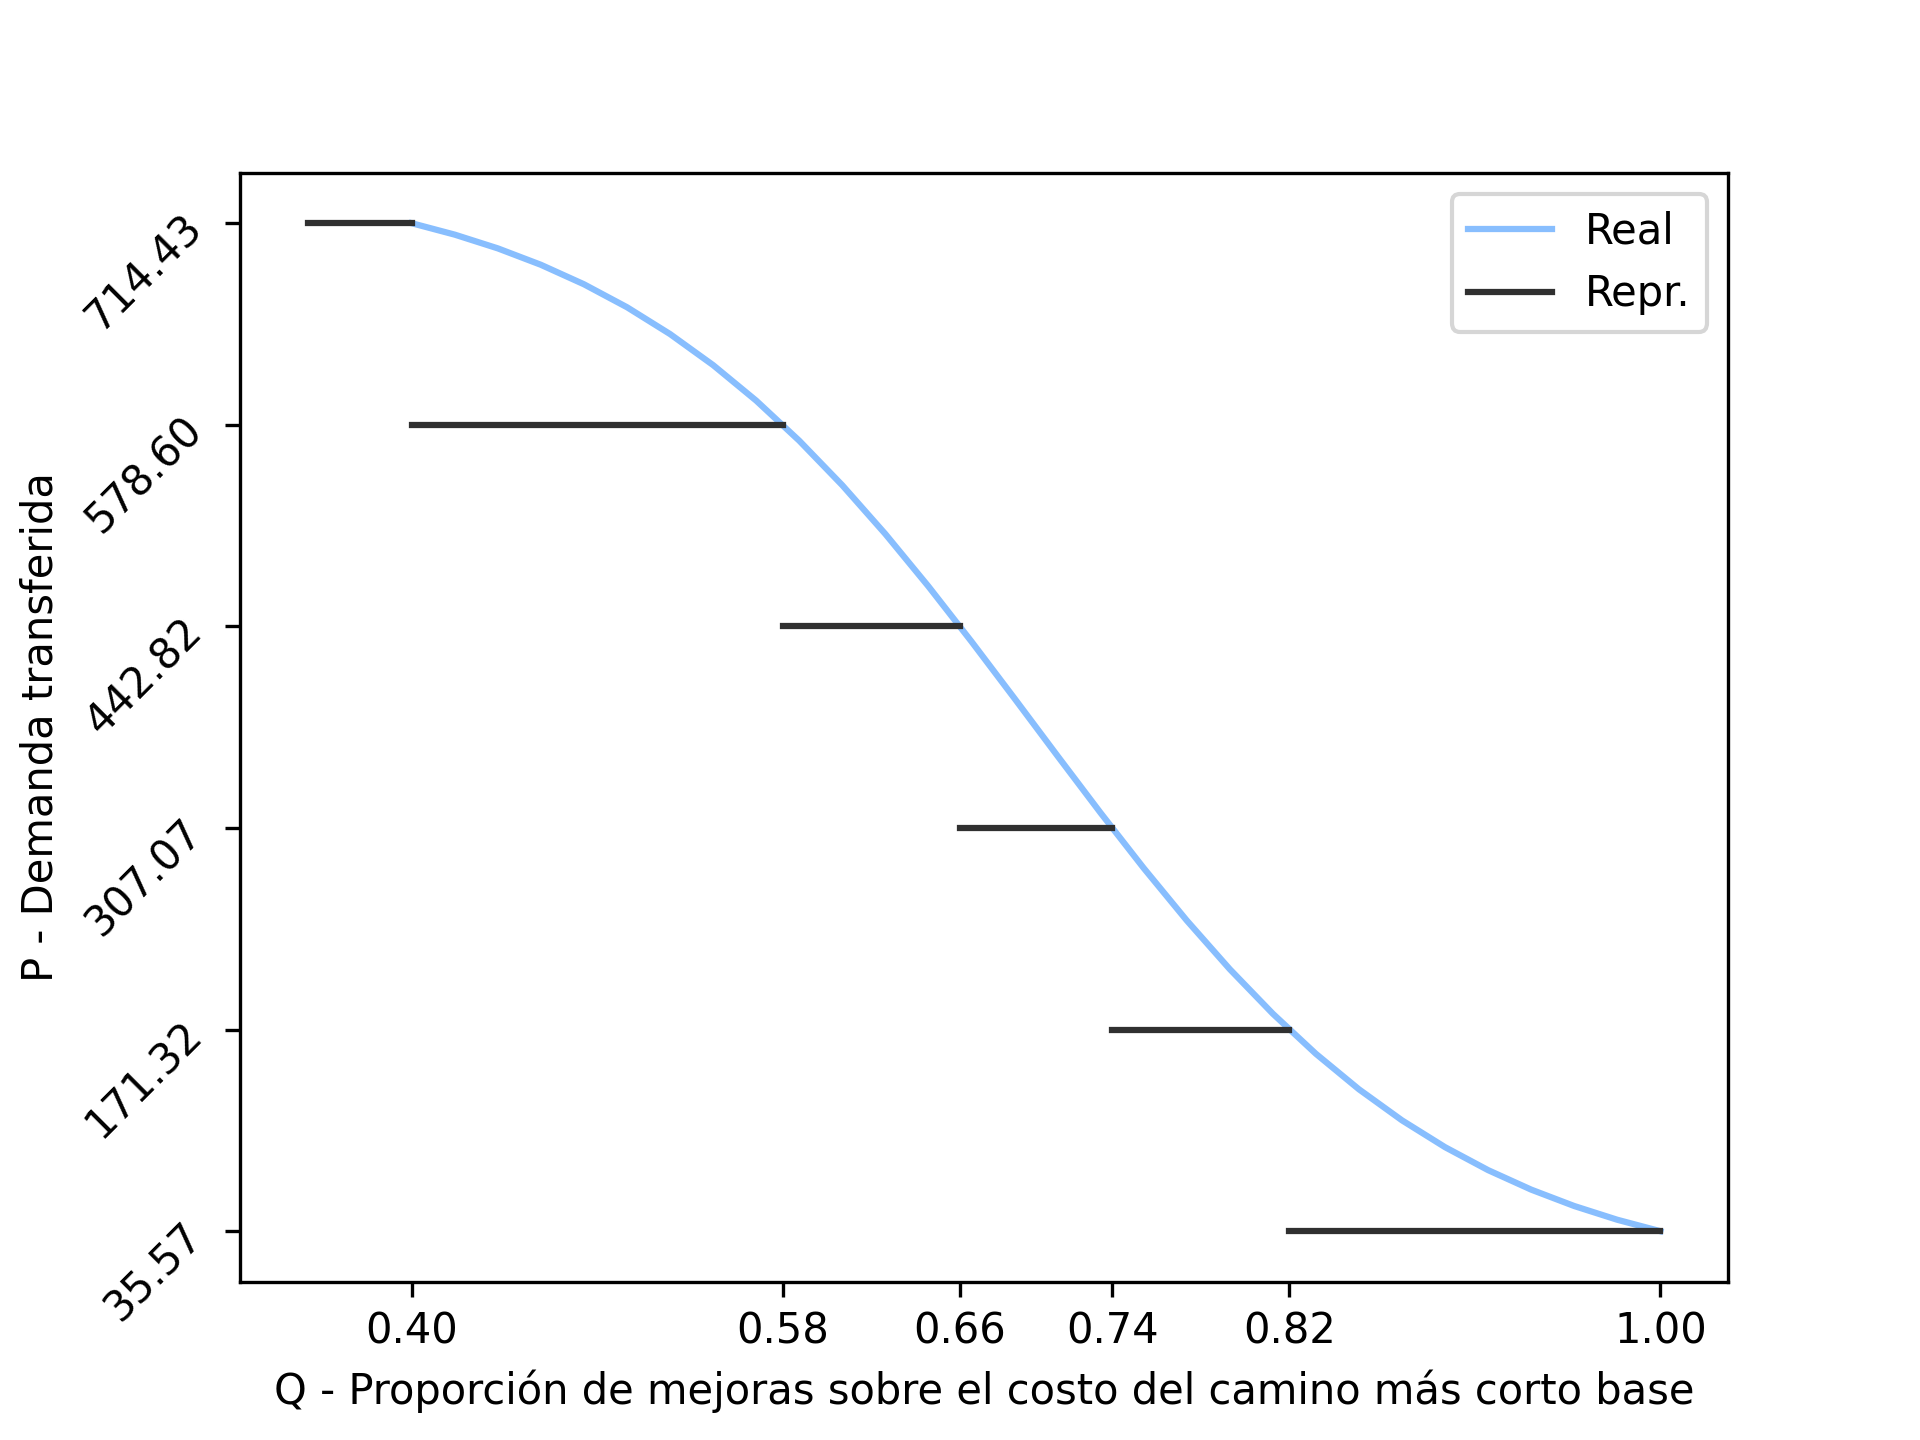
\includegraphics[width=1.1\textwidth]{../resources/f_example.png}
    \end{columns}
\end{frame}

\begin{frame}
    \frametitle{Resolución - Multiobjetivos}

    \begin{columns}[T]
        \column{.5\textwidth}
            \begin{block}{v1}
                Maximizar la demanda transferida y la diferencia entre el punto de quiebre activo y el costo del camino de menor costo (variable r) para cada par OD.
            \end{block}
            \begin{block}{v2}
                Maximizar la demanda transferida y el opuesto del costo del camino de menor costo, para cada par OD.
            \end{block}
        \column{.5\textwidth}
            Ejemplo

            \vspace{.5cm}
            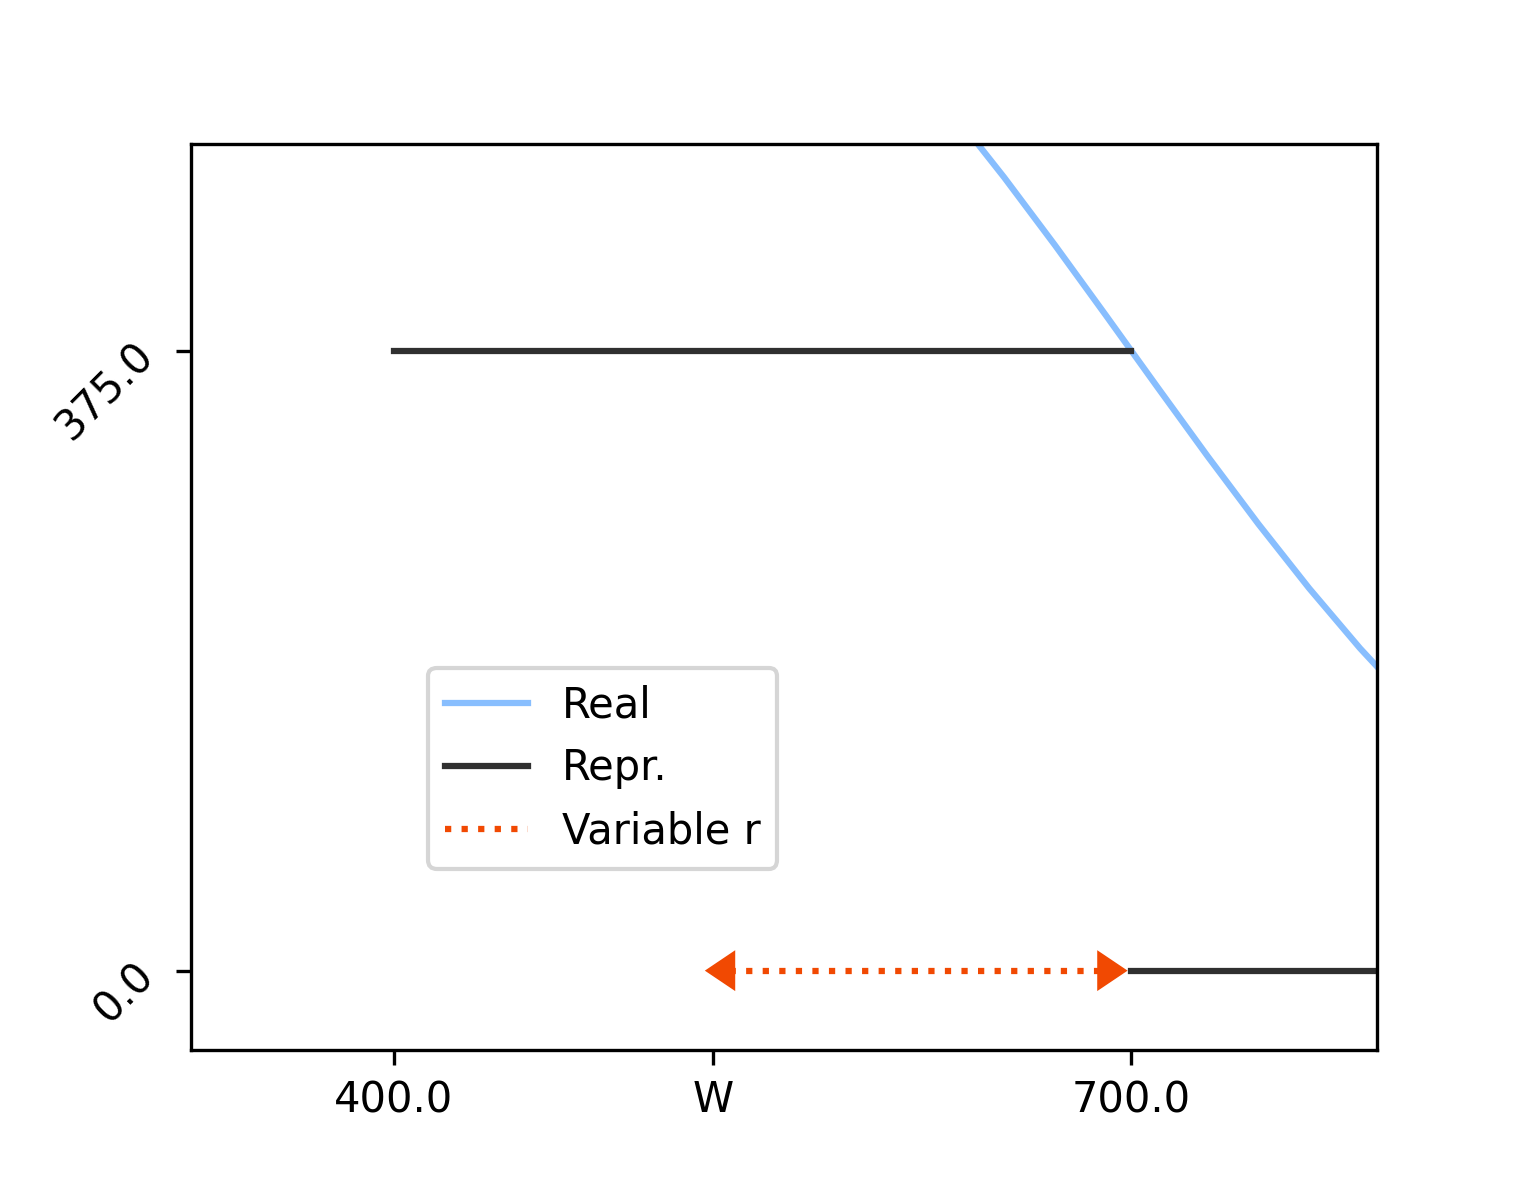
\includegraphics[width=1.1\textwidth]{images/r_visualization.png}
    \end{columns}
\end{frame}

\begin{frame}
    \frametitle{Resolución - Comparativa y validación}

    \begin{itemize}
        \item{De las variantes, buscamos la correctitud en términos de resultados (demanda transferida y ciclovía)}
        \item{De las variantes correctas, buscamos la más rápida}
        \item{La correctitud la verificamos de dos formas:
             \begin{enumerate}
                \item{En términos de la demanda transferida contra una versión de un único objetivo}
                \item{En términos de las propiedades de una solución:
                    \begin{enumerate}
                        \item{Los flujos sobre la red resultante se trasladan por el camino de menor costo}
                        \item{El presupuesto excedente no es suficiente para disminuir el costo de algún camino}
                        \item{La demanda transferida es acorde al costo de usuario sobre la red}
                    \end{enumerate}
                }
            \end{enumerate}
        }
    \item{Ajuste de pesos relativos de multiobjetivos}
    \end{itemize}
\end{frame}

\begin{frame}
    \frametitle{Resolución - Comparativa y validación (cont.)}

    \begin{itemize}
        \item{Dos rondas de 1000 instancias aleatorias sobre la red de Sioux-Falls}
        \item{Solver CBC ejecutado en el ClusterUY}
        \item{Las versiones multiobjetivo fueron correctas luego de ajustes}
        \item{Hubieron diferencias claras en tiempos de ejecución entre las versiones
            del modelado de las funciones de transferencia pero no tanto entre las
            versiones multiobjetvio}
    \end{itemize}
\end{frame}

\section{Resultados experimentales}

\begin{frame}
    \frametitle{Resultados experimentales - Relevamiento de parámetros}

    Relevamos datos específicos del problema:

    \begin{itemize}
        \item{Costo de usuario y de construcción por tipo de ciclovía basado en el estándar BLOS \parencite{blos2007}}
        \item{Funciones de transferencia de demanda: lineal, logística \parencite{shwe2014, ortuz2011}}
        \item{Valores de presupuesto: entre 10\% y 40\% de la red de calles \parencite{rios2015, shwe2014}}
    \end{itemize}
\end{frame}

\begin{frame}
    \frametitle{Resultados experimentales - Sensibilidad de parámetros}

    ¿Cómo afectan los parámetros específicos del problema a las soluciones?

    Utilizamos la red de Sioux-Falls y matriz de demanda tomada de \textcite{Liu2019}. Observamos que:

    \begin{itemize}
        \item{Mayor presupuesto y cantidad de puntos de quiebre inducen mayor transferencia de demanda}
        \item{Variar la función de transferencia de demanda afecta las decisiones de ubicación y tipos de ciclovías}
        \item{Mayor cantidad de puntos de quiebre induce decisiones más inteligentes en términos de ciclovías}
    \end{itemize}
\end{frame}

\begin{frame}
    \frametitle{Resultados experimentales - Sensibilidad de parámetros (cont.)}

    Demanda transferida (en \%) según función y cantidad de puntos de quibre a presupuesto de 40\%.

    \begin{center}
        \begin{tabular}{c c c c c}
               & & \multicolumn{3}{c}{Puntos de quiebre} \\
               \cline{3-5}
               & & 5 & 20 & 50 \\
               \cline{3-5}
               \cline{3-5}
               \multirow{4}{*}{\shortstack{Función de \\ transferencia}}
               & \multicolumn{1}{|c|}{concavidad +} & 40 & 44 & 47 \\
               & \multicolumn{1}{|c|}{logística}    & 44 & 50 & 54 \\
               & \multicolumn{1}{|c|}{lineal}       & 48 & 55 & 57 \\
               & \multicolumn{1}{|c|}{concavidad -} & 72 & 81 & 83 \\
        \end{tabular}
    \end{center}
\end{frame}

\begin{frame}
    \frametitle{Resultados experimentales - Ciudad de Montevideo}

    \begin{itemize}
        \item{1,8 millones de personas}
        \item{4,2 millones de viajes diarios de los cuales el 2,6\% realizado en bicicleta \parencite{Mauttone2017a}}
        \item{1,27\% de la red de calles está cubierta por ciclovías de tres tipos, datos del 2019}
    \end{itemize}
    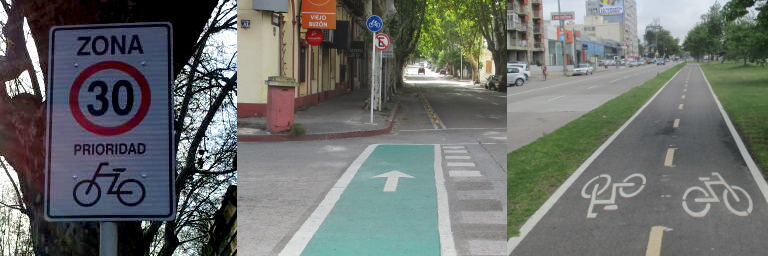
\includegraphics[width=\textwidth]{images/mdeo_tipos_ciclovias.png}
\end{frame}

\begin{frame}
    \frametitle{Resultados experimentales - Ciudad de Montevideo (2)}

    \begin{itemize}
        \item{Prueba sobre una red simplificada de la red de calles de la ciudad (Proyecto CSIC)}
        \item{Datos de demanda del transporte público STM
            \parencite{Massobrio2020}}
        \item{varias ejecuciones:
            \begin{itemize}
                \item{Funciones de transferencia lineal y logística}
                \item{Factores de presupuesto 5\%, 10\%, 40\%, 80\% y 160\% representadas por 10 puntos de quiebre}
                \item{3 tecnologías de ciclovías especializadas}
                \item{Costos de usuarios y de construcción estimados basados en la distancia de los arcos}
            \end{itemize}
        }
    \end{itemize}
\end{frame}

\begin{frame}
    \frametitle{Resultados experimentales - Ciudad de Montevideo (3)}

    Utilizamos datos de STM del año 2015:
    \begin{columns}[T]
        \column{.5\textwidth}
        \begin{itemize}
            \item{Relevados de la utilización de tarjetas STM}
            \item{9.7 millones de viajes mensuales, de los cuales consideramos 6,5 millones en nuestra zonificación}
            \item{Concentración de la demanda hacia la misma región de la red}
        \end{itemize}
        \column{.5\textwidth}
            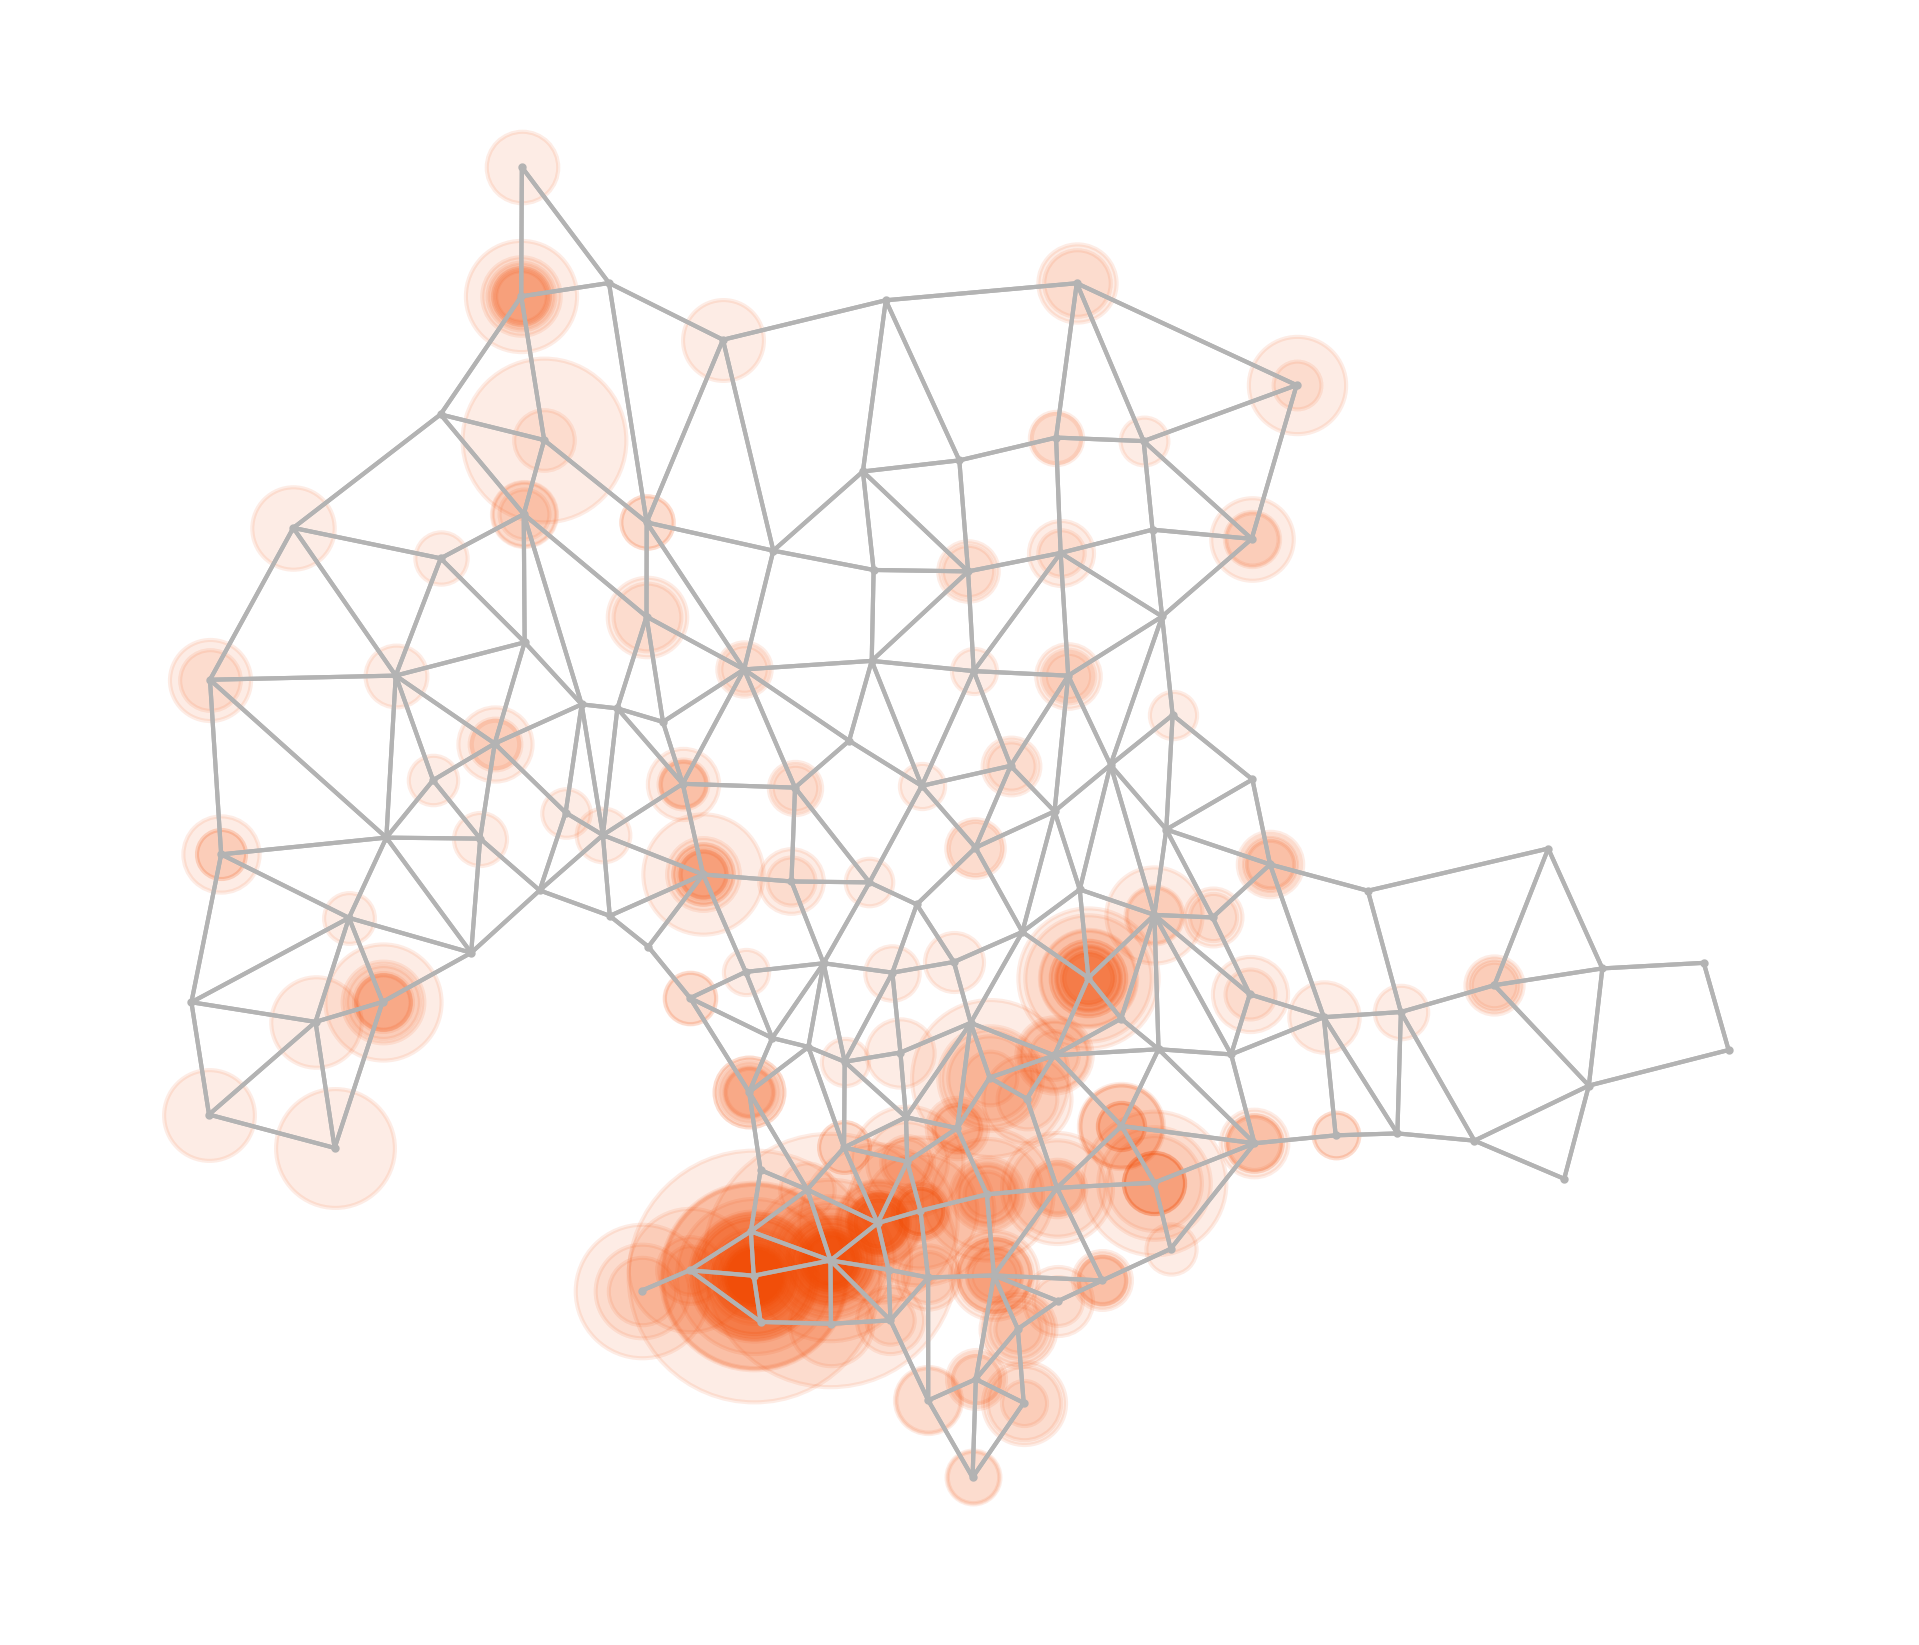
\includegraphics[width=\textwidth]{images/mdeo_demand_topN.png}
    \end{columns}
\end{frame}

\begin{frame}
    \frametitle{Resultados experimentales - Ciudad de Montevideo - Resultados}

    \begin{itemize}
        \item{Poca diferencia entre diferentes funciones de transferencia de demanda}
        \item{Alto impacto en demanda transferida con bajos niveles de presupuesto}
    \end{itemize}

    Para función de transferencia lineal:
    \begin{center}
        \begin{tabular}{c c}
            \hline
            Factor de presupuesto & Demanda transferida \\
            \hline
            \hline
            5  \% & 15,8 \% \\
            10 \% & 24,4 \% \\
            40 \% & 53,9 \% \\
            80 \% & 74,7 \% \\
            160\% & 94,7 \% \\
            \hline
        \end{tabular}
    \end{center}
\end{frame}

\begin{frame}
    \frametitle{Resultados experimentales - Ciudad de Montevideo - Resultados (2)}

    Efectos de la concentración de la demanda en la misma región de la red:

    \begin{itemize}
        \item{Las ciclovías se concentran en dicha región por lo que es menos equitativa}
        \item{Bajos niveles de presupuesto tienen impacto considerable en demanda transferida}
    \end{itemize}

    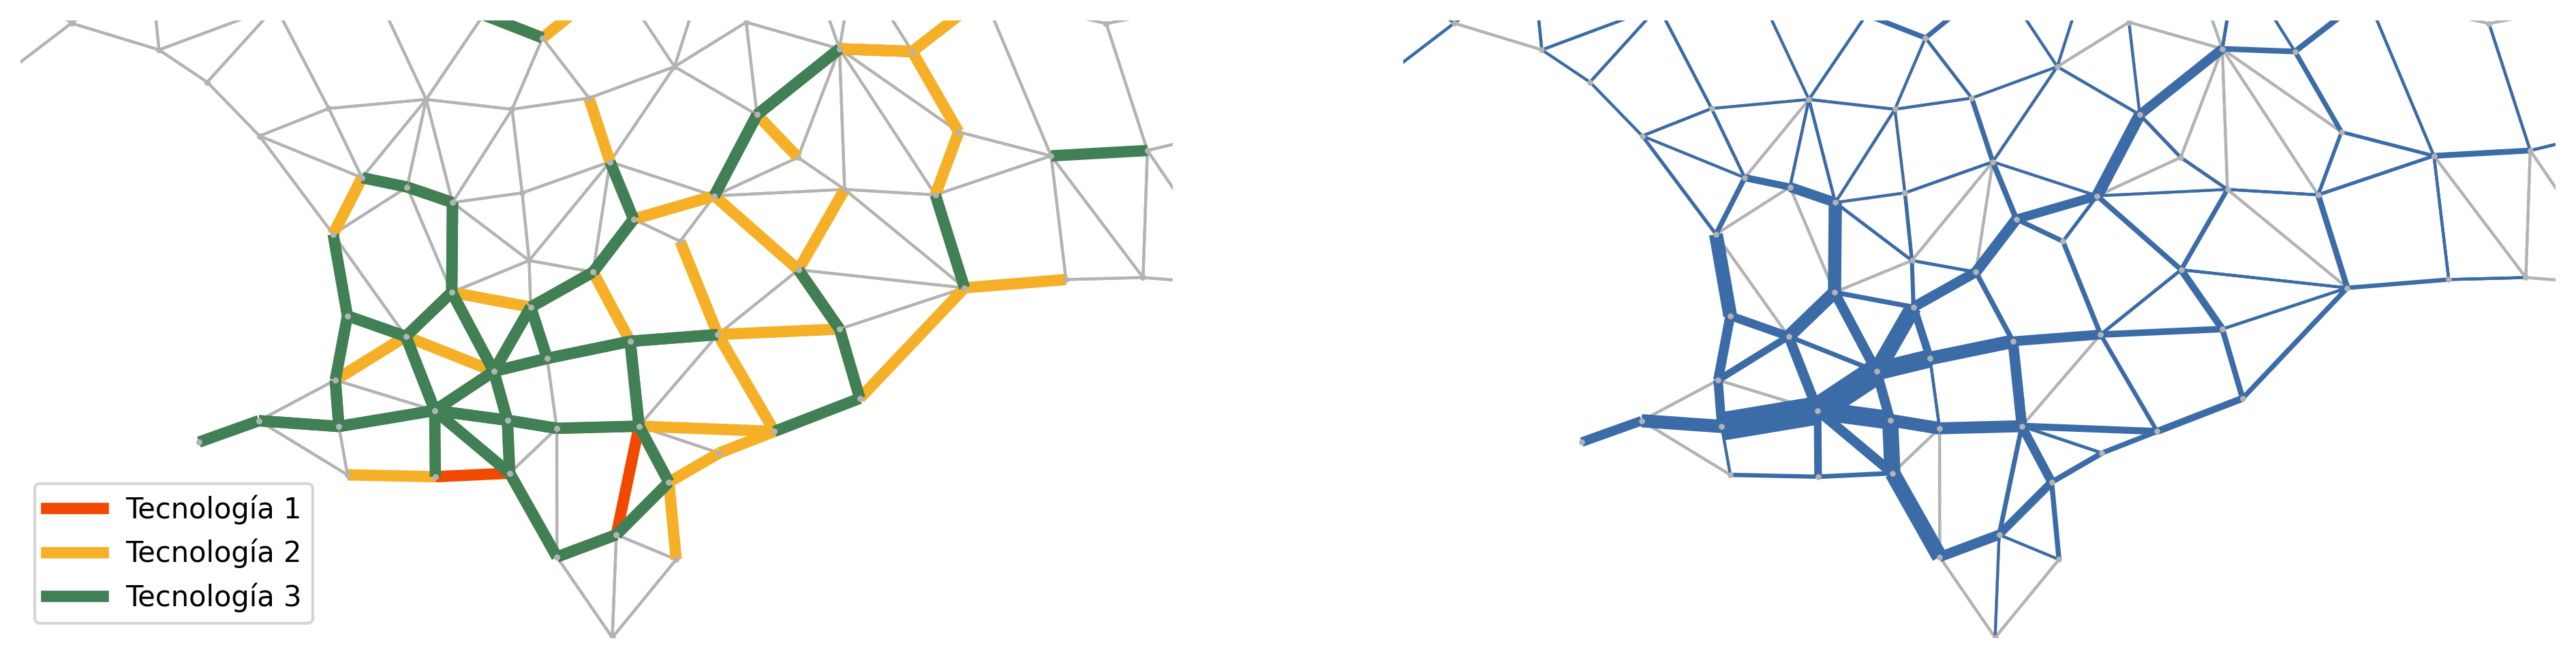
\includegraphics[width=\textwidth]{images/mdeo_0.4_results.png}
    \small
    Ejemplo: ciclovías y flujos para función de transferencia lineal y presupuesto de 40\%.
\end{frame}

\begin{frame}
    \frametitle{Resultados experimentales - Ciudad de Montevideo - Ejecuciones}

    \begin{itemize}
        \item{Solver CPLEX 20.1.0.0, última versión disponible}
        \item{Ejecuciones en el ClusterUY con 16 CPUs, 180 GB de memoria y hasta 5 días de tiempo de ejecución}
        \item{Límites encontrados al incrementar los parámetros de pares OD considerados o tecnologías de ciclovías consideradas:
            \begin{itemize}
                \item{Incrementos en parámetros del problema excedían el límite en memoria disponible}
                \item{En algunos casos el límite de 5 días de ejecución fue alcanzado sin un buen resultado}
            \end{itemize}
        }
    \end{itemize}
\end{frame}

\begin{frame}
    \frametitle{Resultados experimentales - Ciudad de Montevideo - Conclusiones}

    \begin{itemize}
        \item{Poca diferencia entre funciones de transferencia logística y lineal}
        \item{Concentración de inversión en ciclovía sigue la distribución topológica de la demanda}
        \item{Concentración de la demanda permite alto impacto con baja inversión}
        \item{Tiempos de ejecución razonables para las instancias resueltas}
    \end{itemize}
\end{frame}

\section{Conclusiones}

\begin{frame}
    \frametitle{Conclusiones}

    \begin{itemize}
        \item{Modelo basado en conceptos del estado del arte en el diseño de redes}
        \item{Aplicable a instancias grandes (aunque simplificadas)}
        \item{Es posible construir una red de ciclovías que atraiga demanda desde otros medios, basado en datos fundados}
        \item{Sobre el proceso:
            \begin{itemize}
                \item{Transformación del problema binivel a un MILP utilizando características estructurales particulares}
                \item{Durante el trabajo utilizamos varios solvers de código libre (GLPK y CBC) pero su desempeño dista mucho de CPLEX}
            \end{itemize}
        }
    \end{itemize}

\end{frame}

\begin{frame}
    \frametitle{Trabajo a futuro}

    \begin{itemize}
        \item{Posibles extensiones del modelo se pueden basar en los conceptos vistos de otros trabajos de diseños de ciclovías}
        \item{Para instancias más grandes: usar metaheurísticas o algoritmos de descomposición}
        \item{Ejecución con datos relevados específicamente en el marco de una aplicación real del modelo}
        \item{Cuantificar otros aspectos del incremento del uso de la bicicleta:
            impacto en el tráfico,
            impacto en la velocidad del transporte público,
            gasto en mantenimiento de calles
        }
    \end{itemize}
\end{frame}

\end{document}
